% Straight up stealing preamble from Eli Holmes 
%%%%%%%%%%%%%%%%%%%%%%%%%%%%%%%%%%%%%%START PREAMBLE THAT IS THE SAME FOR ALL EXAMPLES
\documentclass{article}

%Required: You must have these
\usepackage{Sweave}
\usepackage{graphicx}
\usepackage{tabularx}
\usepackage{hyperref}
\usepackage{natbib}
\usepackage{pdflscape}
\usepackage{array}
\usepackage{gensymb}
%\usepackage[backend=bibtex]{biblatex}
%Strongly recommended
  %put your figures in one place
%\SweaveOpts{prefix.string=figures/, eps=FALSE} 
%you'll want these for pretty captioning
\usepackage[small]{caption}

\setkeys{Gin}{width=0.8\textwidth}  %make the figs 50 perc textwidth
\setlength{\captionmargin}{30pt}
\setlength{\abovecaptionskip}{10pt}
\setlength{\belowcaptionskip}{10pt}
% manual for caption  http://www.dd.chalmers.se/latex/Docs/PDF/caption.pdf

%Optional: I like to muck with my margins and spacing in ways that LaTeX frowns on
%Here's how to do that
 \topmargin -1.5cm        
 \oddsidemargin -0.04cm   
 \evensidemargin -0.04cm  % same as oddsidemargin but for left-hand pages
 \textwidth 16.59cm
 \textheight 21.94cm 
 %\pagestyle{empty}       % Uncomment if don't want page numbers
 \parskip 7.2pt           % sets spacing between paragraphs
 %\renewcommand{\baselinestretch}{1.5} 	% Uncomment for 1.5 spacing between lines
\parindent 0pt% sets leading space for paragraphs
\usepackage{setspace}
%\doublespacing

%Optional: I like fancy headers
%\usepackage{fancyhdr}
%\pagestyle{fancy}
%\fancyhead[LO]{How do climate change experiments actually change climate}
%\fancyhead[RO]{2016}
 
%%%%%%%%%%%%%%%%%%%%%%%%%%%%%%%%%%%%%%END PREAMBLE THAT IS THE SAME FOR ALL EXAMPLES

%Start of the document
\begin{document}

%\SweaveOpts{concordance=TRUE}
 \bibliographystyle{/Users/aileneettinger/citations/Bibtex/styles/amnat.bst}
\title{Spatial and temporal shifts in photoperiod with climate change} % perspective paper for OSPREE analyses

\author{A.K. Ettinger, D. Buonaiuto, C. Chamberlain, I. Morales-Castilla, E. Wolkovich}
%\date{\today}%do we need to also add any of the following: D. Flynn, T. Savas, J. Samaha, E. Forrestel? 
\maketitle  %put the fancy title on
%\tableofcontents      %add a table of contents
%\clearpage
%%%%%%%%%%%%%%%%%%%%%%%%%%%%%%%%%%%%%%%%%%%%%%%%%%%

%%%%%%%%%%%%%%%%%%%%%%%%%%%%%%%%%%%%%%%%%%%%%%%%%%%
\iffalse
Take-home messages 
(*) Temporal shifts are expected to have a major impact on experienced photoperiod, thus testing for the importance of photoperiod to phenology and adding it to such models should be a major goal.
(*) Current experiments often go well beyond the expected spatial and temporal shifts of climate change, especially for the bigger treatments (Fig. 3) but  the smaller treatments seem to overlap with potential shifts (?!) and appear relevant (Fig. 4-5). 
Could/should we add: 

(*) How to predict how much photoperiod matters? Evidence suggests it varies (importantly?) by ... species, lifestage, photoperiod (Fig. 6), population (that is genotype, and this may relate to latitude). 

More on models ....
In my mind there are two extremes: statistical models and process-based models. Most statistical models have a little process (that's your predictor variables) and most process-based models have a good dose of statistical (you fit the parameters!). I am thinking most SDMs are statistical so you could toss them as an example under the statistical.

To date in statistical models many people either ignore photoperiod or they put it in in some very painful way ('we added photoperiod experienced on the day of budburst to the PEP725 data to test for the role of photoperiod') that is not well designed. What we're fundamentally suggesting is they step a little in the direction of process-based models and:
(1) Use experimental data (there's lots we have shown in this paper) to test if their species or a congeneric species shows a photoperiod effect (ideally test how it varies by lifestage and genotype)
(2) If there is a response, add this to the model (we could cite some of Isabelle's papers to describe how much it could matter).
(3) What will be critical are non-linearities and/or variations across species, lifestages, and populations -- these could fundamentally shape future species and communities! We could help the reader visualize an example of this.
(4) Models ideally will then guide experiments to test some of the critical predictions ....
	
\fi
%%%%%%%%%%%%%%%%%%%%%%%%%%%%%%%%%%%%%%%%%%%%%%%%%%%


%%%%%%%%%%%%%%%%%%%%%%%%%%%%%%%%%%%%%%%%
\iffalse
Nacho's comments 10 October 2018

Not sooo much to add to Lizzie's super helpful comments at this stage. Thanks Ailene for putting this together, 
reading it still makes me very excited about the topic, but perhaps we can still make it more appealing. Just a couple comments:
	

- I agree that we should restrict to plants in the intro and leaving the overview of how this paper may be 
important for other taxa to the end. 

- We say that photoperiod matters but not why it matters. Perhaps we should mention that, one reason why photoperiod would matter to plants is that it is directly related with the amount
of photosynthesis a plant can do, thus influencing physiological processes such as growth. This is obviously
important to plants and yet, commonly overlooked in forecasts. We can try to mention this in a non-text book fashion. 
\fi
%%%%%%%%%%%%%%%%%%%%%%%%%%%%%%%%%%%%%%%%%%%%%%%%%%%


\section*{Introduction}
\par Photoperiod is a critical cue used by plants to synchronize their activities with seasonal climatic changes \citep[e.g.,][]{Hsu:2011,Singh:2017,Basler:2012}. Variation in daylength affects many aspects of plant performance, from growth and reproduction to dormancy and senescence.  Photoperiod represents a reliable cue because it is consistent across years, especially compared to other seasonal cues such as temperature and precipition \citep{saikkonen2012}. 
. For example, relying on photoperiod, rather than temperature alone, may prevent a plant from leafing out during a ``false spring" event (an unusually warm period during winter that is followed by a return of cold temperatures) %Cat- could you one or more relevant references about false springs?

\par  For decades, photoperiod as a cue for woody plant phenology has been studied through growth chamber experiments.  These experiments often  manipulate photoperiod to address basic questions about how photoperiod interacts with temperature to act as a biological cue. Thus temperature, including chilling () and forcing (), is often altered in addition to photoperiod \citep[e.g.,][]{Campbell:1975aa,HEIDE:1977aa,Falusi:1990aa,Spann:2004aa,Laube:2014a}. 

\par Despite the fact that photoperiod is known to be an important cue for plant activity, it is often ignored in forecasts of biological responses to climate change (not sure we want something like this Figure \ref{fig:wos}). This may be problematic because, although photoperiod itself is stable over time, the photoperiod that species \emph{experience}, as they undergo climate change-induced shifts in space and time, is likely to be much less stable. With recent warming, many species have shifted their distributions poleward and upward in elevation (i.e., range shifts, ADD CITATIONS), and/or shifted their activity earlier in the year (i.e., phenological shifts, CITATIONS). These spatial and temporal shifts will alter the photoperiod regime experienced by organisms. 


\par Here, we ask: 
\begin{enumerate}
\item How will climate change alter the photoperiod experienced by organisms, given observed climate change-induced biological shifts, both spatially and temporally?
\item What are the implications of altered photoperiods for biological responses to climate change?
\item Can the large quantity data from growth chamber experiments altering photoperiod be applied to forecasting biological implications of climate change (i.e., do they occur at the appropriate scale)?
\item What outstanding questions warrant further research to more fully incorporate photoperiod into forecasts of biological effects with climate change?
\end{enumerate}
\par We address these questions using a new database of plant growth chamber studies that manipulate photoperiod and temperature and measure plant responses, including budburst, flowering, and growth. 
\section*{How will climate change alter the photoperiod experienced by organisms?}
\par Species experience different photoperiod regimes depending on their location in space and the seasonal timing of their activity. Spring green-up date, for example, varies with latitude, occurring earlier toward the equator and later toward the poles (Figure \ref{fig:greenup}a). Athough this general pattern is consistent across years (Figure \ref{fig:greenup}b), there is spatial variation: a year that results in early green-up at 35\degree, for instance, may not be an early year at 50\degree latitude(Figure \ref{fig:greenup}c).
\par Against this existing background variation, climate change is likely to cause average shifts in experienced photoperiod, as species respond to wamring temperatures. Spatial shifts in species ranges and temporal shifts in species phenology and activity will alter the photoperiods experienced by organisms with future climate change. The magnitude of these alterations will vary depending on the organism's location and the type of shift(s) it undergoes. For example, poleward shifts in species' ranges cause organisms to experience a wider range of daylength throughout the year (Figure \ref{fig:spacetime}). Elevational shifts, on the other hand, would cause minimal changes in photoperiod throughout the year. 
\par To date, most of the scientific literature has focused on how spatial range shifts with climate change will affect photoperiod \citep{saikkonen2012} (other citations?), but temporal shifts are actually likely to yield bigger changes in experienced photoperiod than spatial shifts (Figure \ref{fig:spacetime}). For example, consider a tree at latitude 45\degree that completes spring budbursts around DOY 91 (April 2), on average. If it's phenology shifts 30 days earlier (i.e., a rate of XX days per degree of warming, as has been observed, Parmesan) it will experience a daylength that is XX hours shorter. However, if the same tree species shifts its range up in latitude 0.5 degrees (i.e., a rate of XX km per degree of warming, as has been observed), it will experience a daylength that is only XX minutes shorter on the same DOY. 

\par In many cases organisms may shift both their geographic ranges and their phenology simulataneously.  Furthermore, photoperiod sensitivity, or the degree to which phenology is controlled by daylength, can also vary with latitude \citep{Howe:1996,saikkonen2012,Partanen:2005aa,Vihera-Aarnio:2006aa,Caffarra:2011b,gauzere2017}. It is unclear how all of these complications will interact to affect the photoperiod experienced by organisms, with future climate change.
\section*{What are the implications of altered photoperiods for biological responses to climate change?}
\par Daylength plays a role in controling critical plant functions, including vegetative growth, cell elongation, budburst, and flowering \citep{Linkosalo:2006aa,erwin1998,sidaway2010, Hsu:2011,Heide:2011aa,Ashby:1962aa,Heide:2012aa}. Climate change-induced shifts in photoperiod are therefore likely to alter these functions. The direction and magnitude of these alterations is likely to vary, however, because the effect of daylength differs across species \citep{Sanz-Perez:2009aa, zohner2016}, lifestage \citep{Partanen:2005aa}, and population (need citations!).  
\par Photoperiod often interacts with temperature to affect phenology. The timing of budburst in woody plants is controlled by interactions between chilling (a critical amount of cold temperatures that must be experienced to break dormancy), forcing (a critical amount of warm temperatures), and daylength \citep{flynn2018,Heide:2008aa, zohner2016}. Over the past century, budburst has shifted earlier in diverse woody species (CITES), a pattern that, to date, can be largely explained by warming temperatures. Photoperiod may eventually become a limiting factor, constraining the ability of species to respond to additional warming \citep{koerner2010b,vitasse2013, Morin:2010aa,Nienstaedt:1966aa}. Interactions between photoperiod, forcing, and chilling could therefore result in muted or exaggerated phenological shifts, compared to what would be expected based on temperature change alone.  "photoperiod cues can dampen phenological advance (Wareing 1956; Ashby et al. 1992; Mimura \& Aitken 2007; Aldrete, Mexal \& Burr
2008; Lopez et al. 2008;  Cooke, Eriksson \& Junttila 2012)." 
(Say something about crossing thresholds of daylength and the "external coincidence model" for photoperiod control \citep{bastow2002,kobayashi2007,andres2012,Singh:2017}?)

\section*{Can existing experiments be applied to improve forecasting?}
\par Current forecasts of biological responses to climate change In some forecasting methods (e.g. species distirbution modelling), the role of photoperiod is largely ignored (i think this is true? add some citations). In other cases, photoperiod is incorporated into foreacasts, along with other variables such as evaporative demand, and temperature \citep [e.g. ED] []{jolly2005, medvigy2013}. These models need to be more widely tested, e.g. in different ecosystems, and across different species and populations. They also need to incorporate recent findings about the role of photoperiod in phenology.     

\par In some cases, experiments manipulate photoperiod at relevant scales (e.g., XXX, Figure \ref{fig:photomap}, Table \ref{table:phototreats}). Many experiments, however, manipulate photoperiod much more dramatically than will occur with climate change (Figures \ref{fig:photomap}, \ref{fig:fagus},\ref{fig:quercus}, but see \citep{Basler:2012}), so it is difficult to extrapolate findings to forecasting. (This may not be true for all latitudes- for example high latitudes experience more dramatic changes in photoperiod across the year.)

\section* {Outstanding questions}
There is a great need to better understand exactly how photoperiod acts as a cue. The divergent effects of photoperiod observed across studies (e.g., Figure \ref{fig:photocurve}) suggests that photoperiod interacts with other environmental drivers, such as chilling and forcing, to affect phenology and other activities. However, exactly how it interacts with temperature to break dormancy, as well as the type of response it ellicits (e.g., linear versus non-linear threshold) is unclear. 

how much does 
model accuracy (process-based or correlational-statistical-SDMs) improve when we account for photoperiod? If 
models do not improve much or not at all, then I guess we could forget about it. However, it is likely that
photoperiod be important for certain taxa, in certain regions and when using certain models, and answering that
is really important, isn't it?

\section*{Conclusions}
Organisms may experience large changes to the photoperiod they experience, under climate change, even if they do not shift their ranges spatially. To incorporate photoperiod into forecasting of climate change responses, more studies are needed with fine-scale changes in photoperiod. 
An altered photoperiod is likely to have implications for a variety of plant responses, given the diverse organisms that rely on daylength to cue their activities \citep[e.g.,][] {mcallan2006,linn1996,Flynn:2018,solbakken1994}.

\section* {To do:}
\begin{enumerate}
\item Update table/map with new column for significance (and perhaps direction of results). also, add 3 ER studies- if they are still there following treatment checks in october 2018.
\end{enumerate}
\section* {Random notes that may be useful to work in somewhere:}
\begin {enumerate}
\item Bradshaw and Holzapfel (2001) showed that the pitcher plant mosquito,
Wyeomyia smithii, has evolved a shorter critical photoperiod in association with a
longer growing season. Northern populations of this mosquito now use a shorter
day-length cue to enter winter diapause, doing so later in the fall than they did
24 years ago.
\item Decreasing day-length is the main environmental cue inducing growth cessation and bud set in many perennial plants, including poplar 
\begin{enumerate}

\item Lagercrantz U: At the end of the day: a common molecular mechanism for photoperiod responses in plants?. J Exp Bot. 2009, 60: 2501-2515. 10.1093/jxb/erp139.
\item Howe GT, Gardner G, Hackett WP, Furnier GR: Phytochrome control of short-day-induced bud set in black cottonwood. Physiol Plant. 1996, 97: 95-103. 10.1111/j.1399-3054.1996.tb00484.x.
\end{enumerate}

\item Response to photoperiod is under strong genetic control %EMW: I think we should weave this in more fully to the paper!
\begin{enumerate}
\item Bradshaw HD, Stettler RF: Molecular genetics of growth and development in Populus. IV. Mapping QTLs with large effects on growth, form, and phenology traits in a forest tree. Genetics. 1995, 139: 963-973.
\item Keller SR, Soolanayakanahally RY, Guy RD, Silim SN, Olson MS, Tiffin P: Climate-driven local adaptation of ecophysiology and phenology in balsam poplar, Populus balsamifera L. (Salicaceae). Am J Bot. 2011, 98: 99-108. 10.3732/ajb.1000317.
\item Weih M: Intensive short rotation forestry in boreal climates: present and future perspectives. Can J Forest Res. 2004, 34: 1369-1378. 10.1139/x04-090.
\end{enumerate}
\end {enumerate}
\bibliography{/Users/aileneettinger/git/ospree/refs/ospreebibplus}
\clearpage
\section* {Tables}
% latex table generated in R 3.5.1 by xtable 1.8-3 package
% Thu Nov  1 14:08:50 2018
\begin{table}[ht]
\centering
\caption{\textbf{Growth chamber experiments and their photoperiod treatments}, compared to the spatial and temporal shifts required for organisms to experiments photoperiod changes equivalent to those treatments. For shifts in space, `ER' indicates that the photoperiod treatments exceeds the change of photoperiod from moving up to 40 degrees latitudinally on June 21. For shifts in time, `ER' indicates that the range of photoperiod treatments exceeds the change in daylengths at that latitude during the entire year. `max NA' indicates that the maximum daylength treatment does not exist at that latitude; `min NA'indicates that the minimum daylength treatment does not exist at that latitude.} 
\label{table:phototreats}
\begin{tabular}{|p{0.18\textwidth}|p{0.15\textwidth}|p{0.08\textwidth}|p{0.08\textwidth}|p{0.08\textwidth}|p{0.06\textwidth}|p{0.06\textwidth}|p{0.12\textwidth}|}
  \hline
idstudy & continent & lat & long & day\_range & delta & space & time \\ 
  \hline
ashby62\_exp1 & north america & 42.99 & -89.41 & 8-16 & 4.00 & 18.2 & min NA (9) \\ 
  basler14\_exp1 & europe & 46.31 & 8.27 & 9.2-16 & 1.00 & 6 & -22 \\ 
  caffarra11b\_exp2 & europe & 52.32 & -6.93 & 10-16 & 2.00 & 7.5 & -30 \\ 
  falusi90\_exp1 & europe & 46.03 & 10.75 & 9-13 & 4.00 & 16 & -82 \\ 
  falusi96\_exp3 & europe & 38.27 & 15.99 & 9-13 & 4.00 & 21.6 & -111 \\ 
  ghelardini10\_exp1 & europe & 43.72 & 11.37 & 8-16 & 8.00 & 21.9 & ER \\ 
  heide05\_exp1 & europe & 56.18 & -4.32 & 10-24 & 14.00 & ER & ER \\ 
  heide08\_exp1 & europe & 48.40 & 11.72 & 10-24 & 14.00 & ER & ER \\ 
  heide11\_exp1 & europe & 59.67 & 10.67 & 10-20 & 10.00 & ER & max NA (18.7) \\ 
  heide12\_exp1 & europe & 56.50 & -3.06 & 10-24 & 5.00 & 8.9 & -64 \\ 
  heide15\_exp2 & europe & 56.50 & -3.06 & 10-15 & 1.00 & 3.2 & -13 \\ 
  heide93\_exp1 & europe & 59.50 & 10.77 & 8-24 & 16.00 & ER & ER \\ 
  heide93a\_exp1 & europe & 59.67 & 10.83 & 8-24 & 16.00 & ER & ER \\ 
  heide93a\_exp3 & europe & 47.50 & 7.60 & 13-16 & 1.00 & 5.7 & -18 \\ 
  howe95\_exp1 & north america & 40.55 & -124.10 & 9-24 & 2.00 & 13.1 & -64 \\ 
  laube14a\_exp1 & europe & 48.40 & 11.71 & 8-16 & 4.00 & 14.3 & -87 \\ 
  myking95\_exp1 & europe & 56.10 & 9.15 & 8-24 & 16.00 & ER & ER \\ 
  nienstaedt66\_exp1 & north america & 44.17 & -103.92 & 8-20 & 12.00 & ER & ER \\ 
  okie11\_exp1 & north america & 32.12 & -83.12 & 0-12 & 12.00 & ER & ER \\ 
  partanen01\_exp1 & europe & 61.93 & 26.68 & 6-16 & 10.00 & ER & -105 \\ 
  partanen05\_exp1 & europe & 61.82 & 29.32 & 5-20 & 5.00 & ER & -67 \\ 
  partanen98\_exp1 & europe & 60.03 & 23.05 & 8.66-12 & 3.34 & 5.1 & -37 \\ 
  pettersen71\_exp1 & europe & 59.66 & 10.77 & 10-24 & 2.00 & 4 & -23 \\ 
  Sanz-Perez09\_exp1 & europe & 40.40 & -3.48 & 10-16 & 6.00 & 23.6 & ER \\ 
  viheraaarnio06\_exp1 & europe & 60.45 & 24.93 & 16-17 & 1.00 & 2.1 & -12 \\ 
  viheraaarnio06\_exp1 & europe & 67.73 & 24.93 & 20-21 & 1.00 & ER & -5 \\ 
  viheraaarnio06\_exp2 & europe & 60.45 & 24.93 & 15-19 & 4.00 & 5.1 & -62 \\ 
  viheraaarnio06\_exp2 & europe & 67.73 & 24.93 & 22-23 & 1.00 & ER & -3 \\ 
  worrall67\_exp 3 & north america & 41.31 & -72.93 & 8-16 & 8.00 & 24.3 & ER \\ 
  zohner16\_Exp1 & europe & 48.16 & 11.50 & 8-16 & 8.00 & ER & ER \\ 
   \hline
\end{tabular}
\end{table}\clearpage
\section* {Figures}
\begin{figure}[p]
\centering
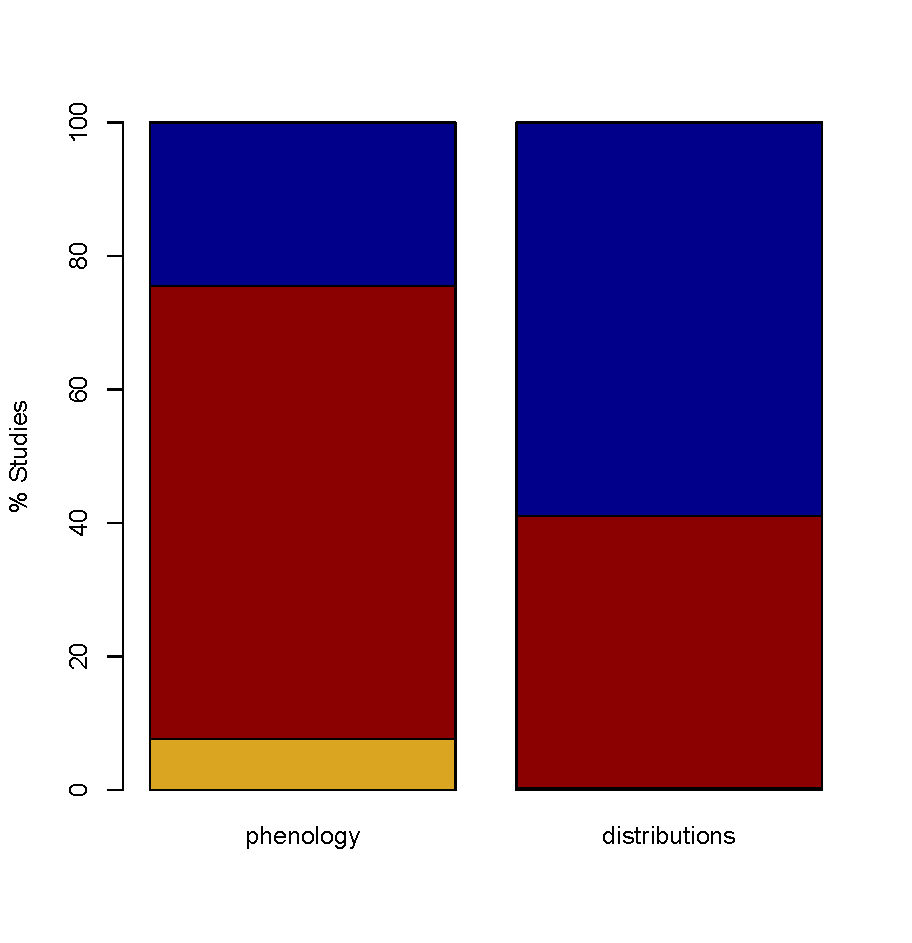
\includegraphics{/Users/aileneettinger/git/ospree/docs/photoperiod/figures/photoperiod_wos.pdf} %
\caption{\textbf{Photoperiod is not a focus of many studies forecasting biological responses to climate change}. Temperature is more often included as a keyword than photoperiod.}
 \label{fig:wos}%
 \end{figure}
 
\begin{figure}[p]
\centering
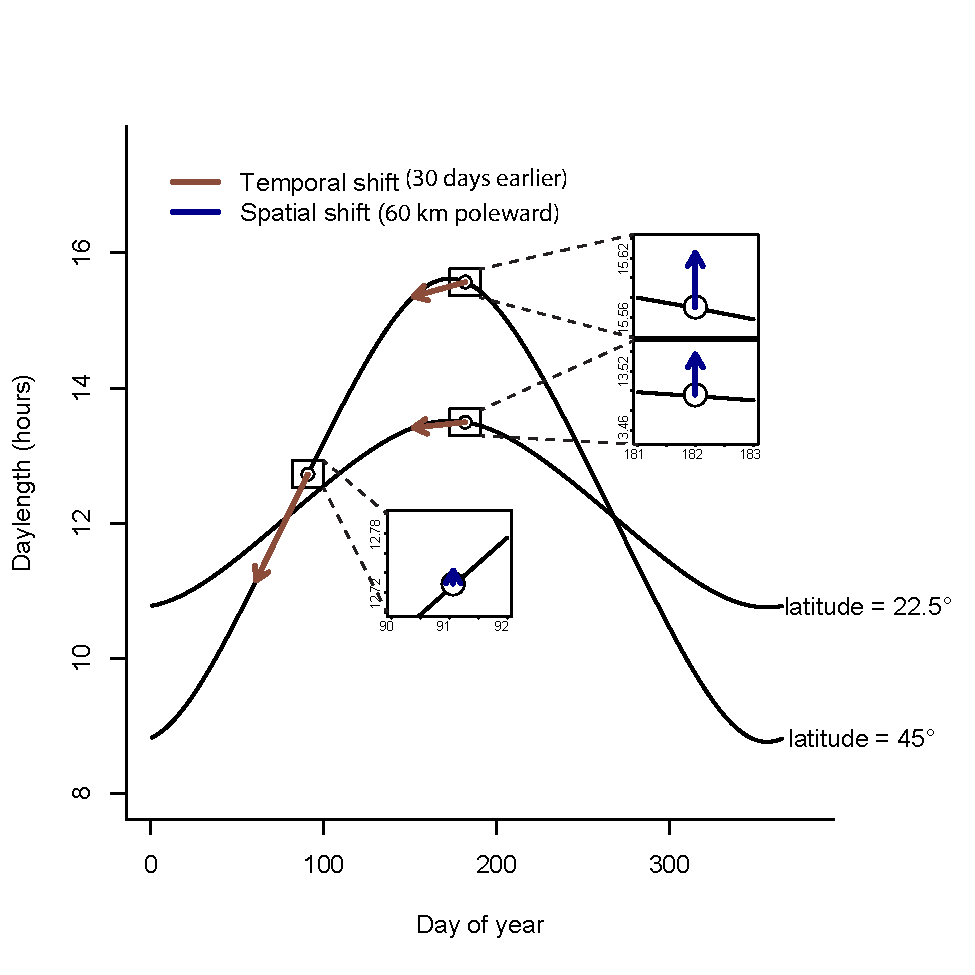
\includegraphics{/Users/aileneettinger/git/ospree/analyses/photoperiod/figures/photo_spacetime_v2.pdf} %
\caption{\textbf{Photoperiod varies with latitude and throughout the year}, such that temporal shifts in activity yield larger changes in experienced photoperiod compared with spatial shifts. Here, we show this variation at two latitudes, using hypothetical rates of spatial and temporal shifts: 30 days earlier for temporal shifts, and 0.5 degrees poleward for spatial shifts. These shifts, which are similar to observed average rates \citep[][e.g.,]{parmesan2006,chen2011}, highlight the greater magnitude in daylength changes close to the equinox (e.g., DOY 91), versus close to the summer solcstice (e.g., DOY 182).}
 \label{fig:spacetime}%
 \end{figure}
 
\begin{figure}[p]
\centering
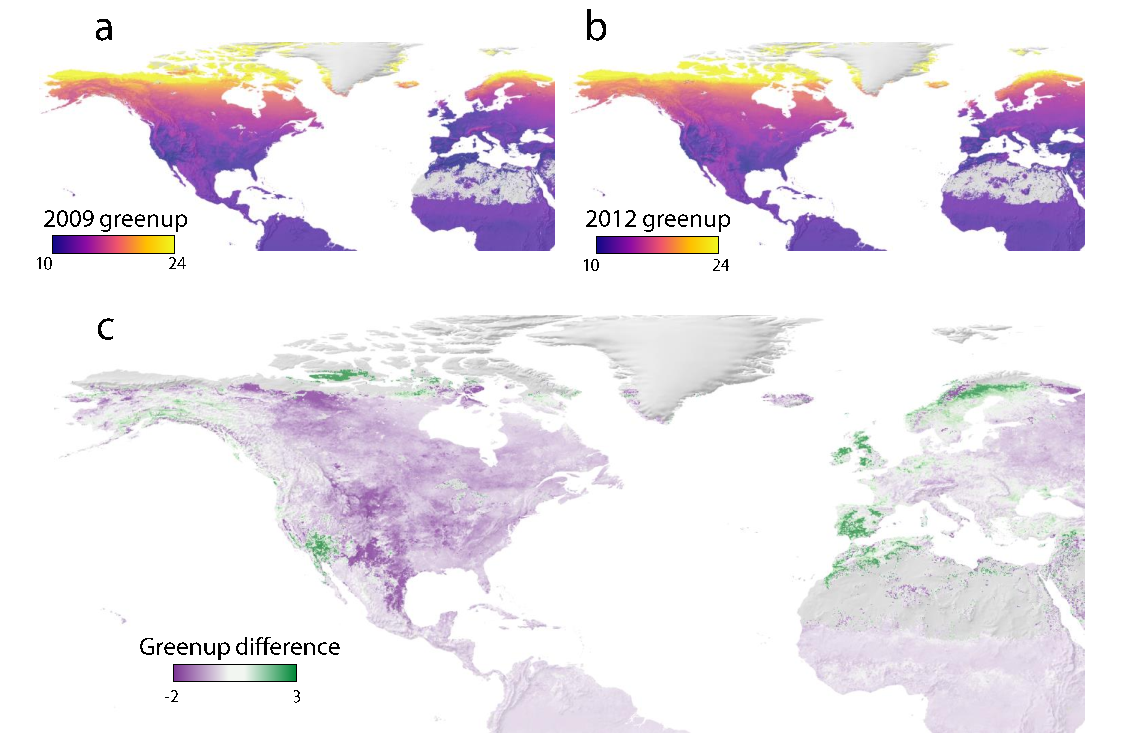
\includegraphics{/Users/aileneettinger/git/ospree/docs/photoperiod/figures/Greenup_corr.pdf} %2009 greenup
\caption{\textbf{The photoperiod on the green up date (start of spring) varies over space} and among years. Hours of daylight on the date of spring green up from MODIS satilite data across North America and Europe for an average (2009, a) and  early (2012,b) North American start of spring. The differences between the years are shown in (c). }
 \label{fig:greenup}%
 \end{figure}
\begin{figure}[p]
\centering
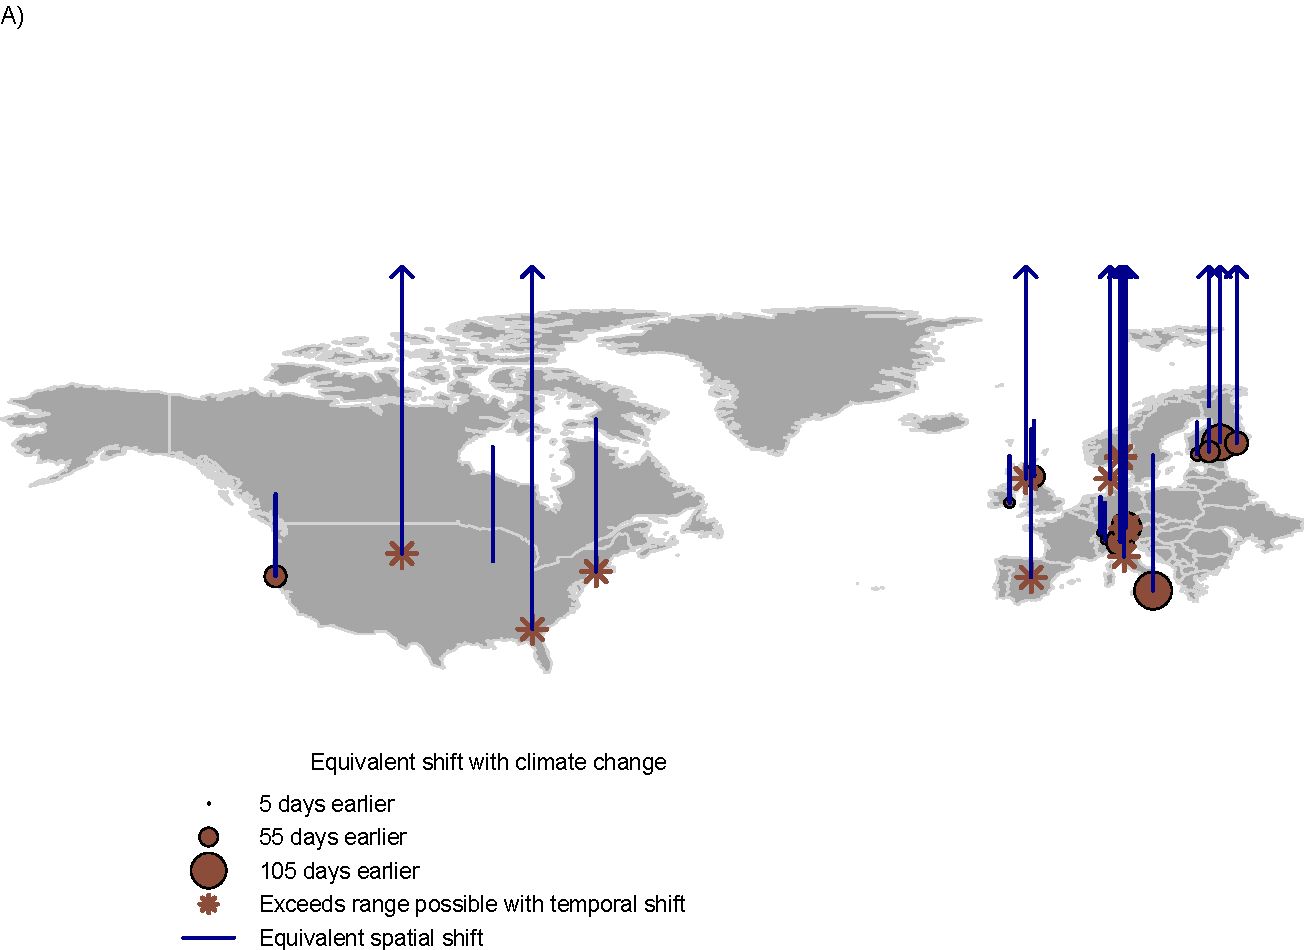
\includegraphics{/Users/aileneettinger/git/ospree/analyses/photoperiod/figures/ospree_photopmap.pdf} 
\caption{\textbf{OSPREE experiments that manipulate photoperiod}, and their equivalent spatial and temporal shifts, mapped (A), and graphed (B-C). Observed rates (dashed gray lines) 16.9 kilometers per decade (or approximately 1.5 degrees in 100 years) for spatial shifts (Chen et al. 2011) and 2.3 days per decade (or 23 days in 100 years) for temporal shifts (Parmesan and Yohe 2003).}
 \label{fig:photomap}
 \end{figure}


 
\begin{figure}[p]
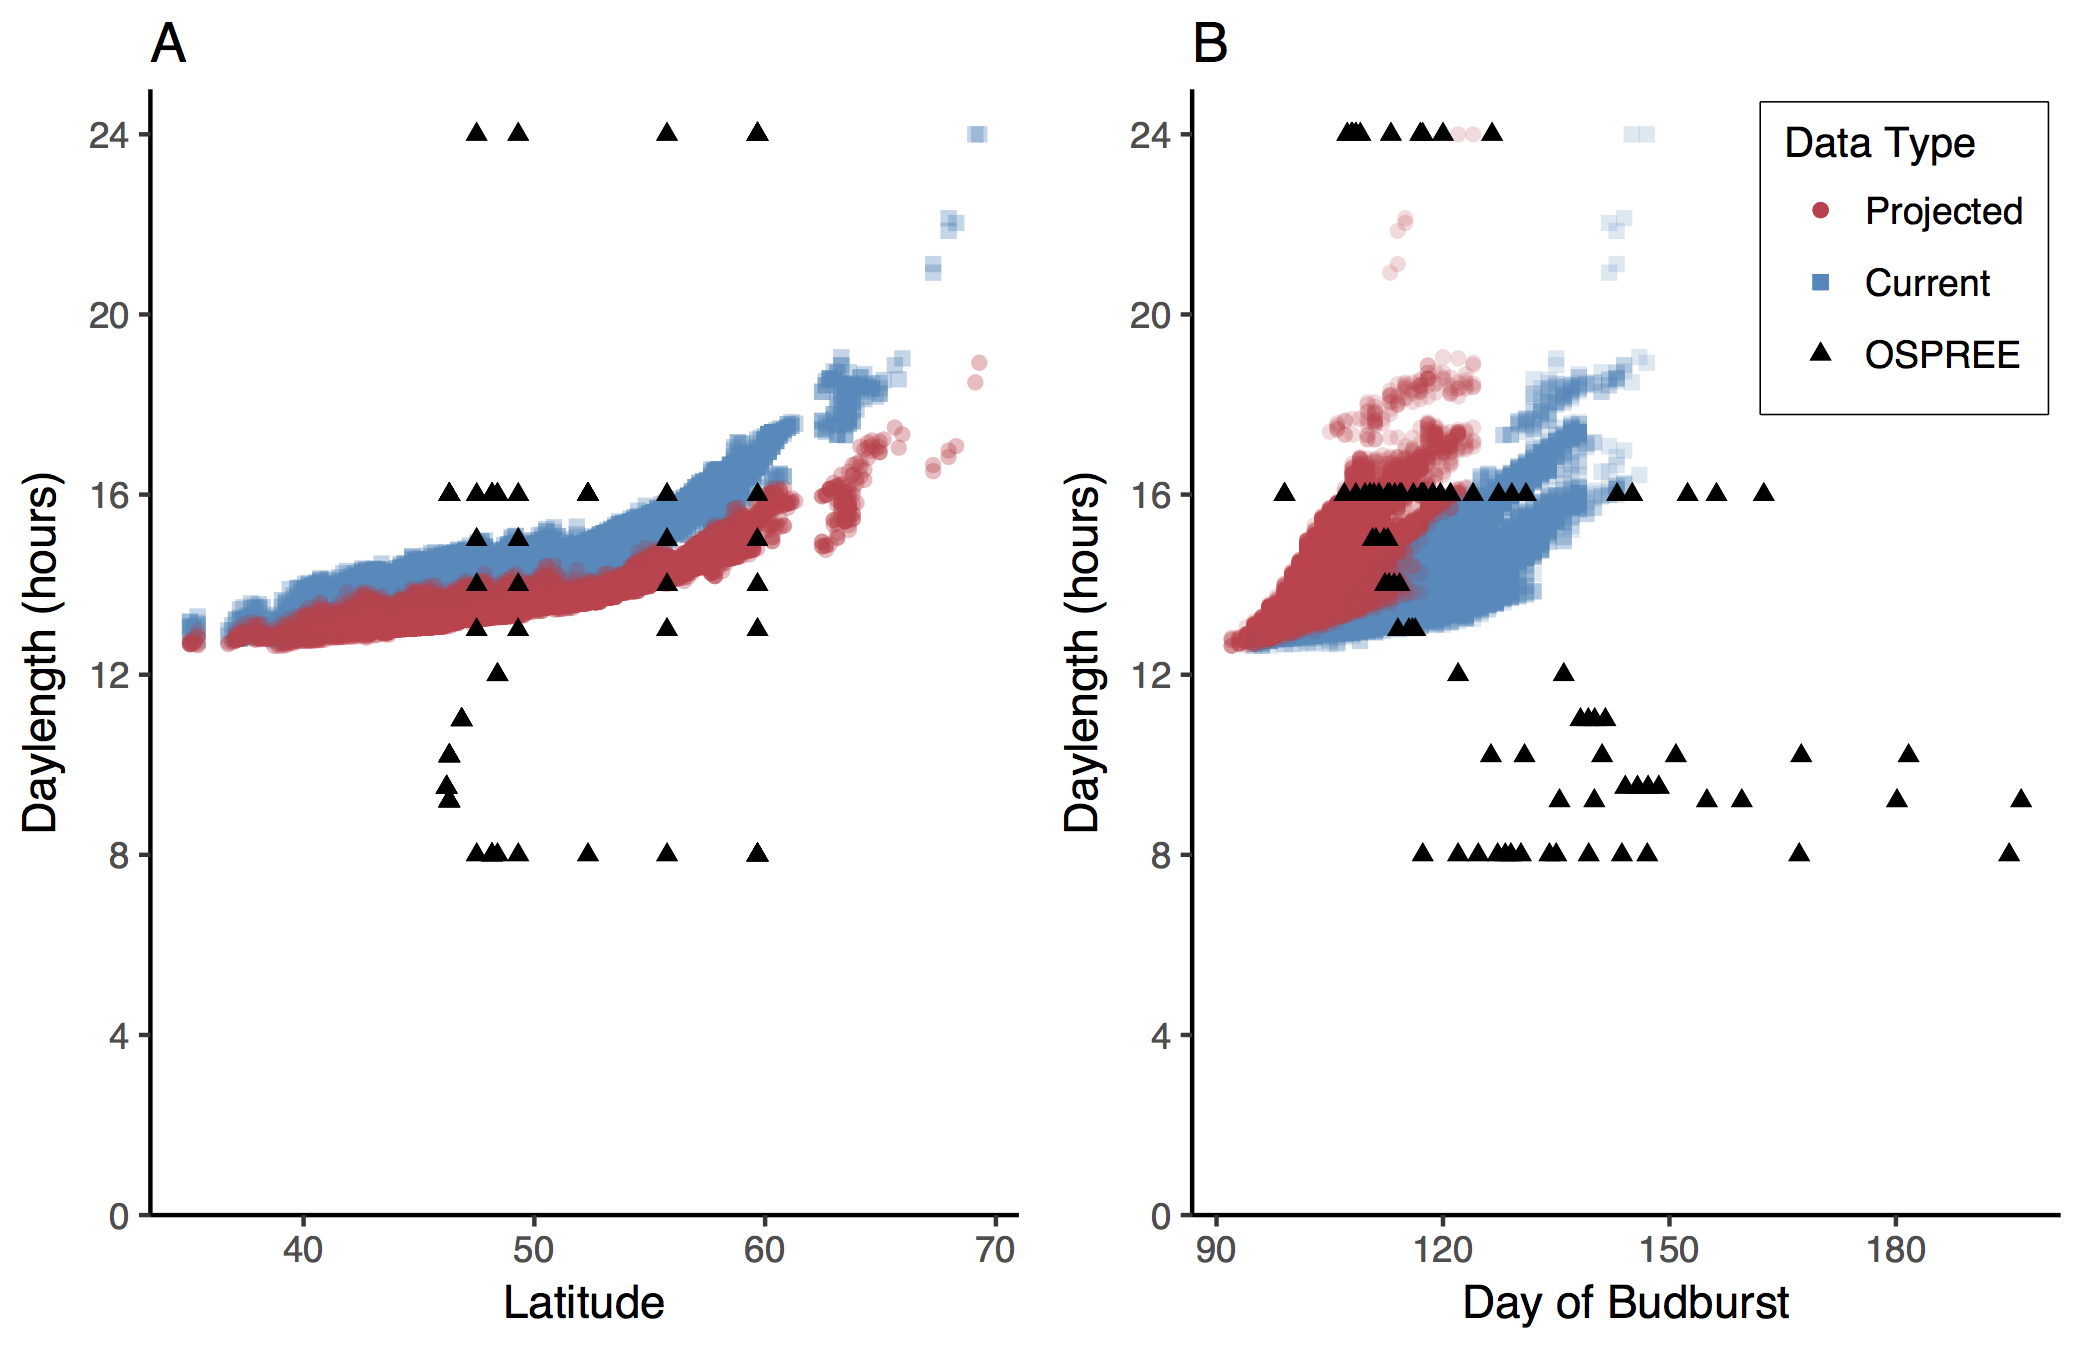
\includegraphics{/Users/aileneettinger/git/ospree/analyses/photoperiod/figures/2D_fagus_actual.png} 
\caption{\textbf{Experimental treatments of daylength in the OSPREE database, shown by latitude (A) and by day of budburst (B)} for \textit{Fagus sylvatica}. For comparison, we show the daylength when budburst occurs in its current and projected ranges (A) and in its current range only, with expected shifts in phenology (B). Estimates and projections are from Phenofit \citep{duputie2015}}
 \label{fig:fagus}
 \end{figure}
 
\begin{figure}[p]
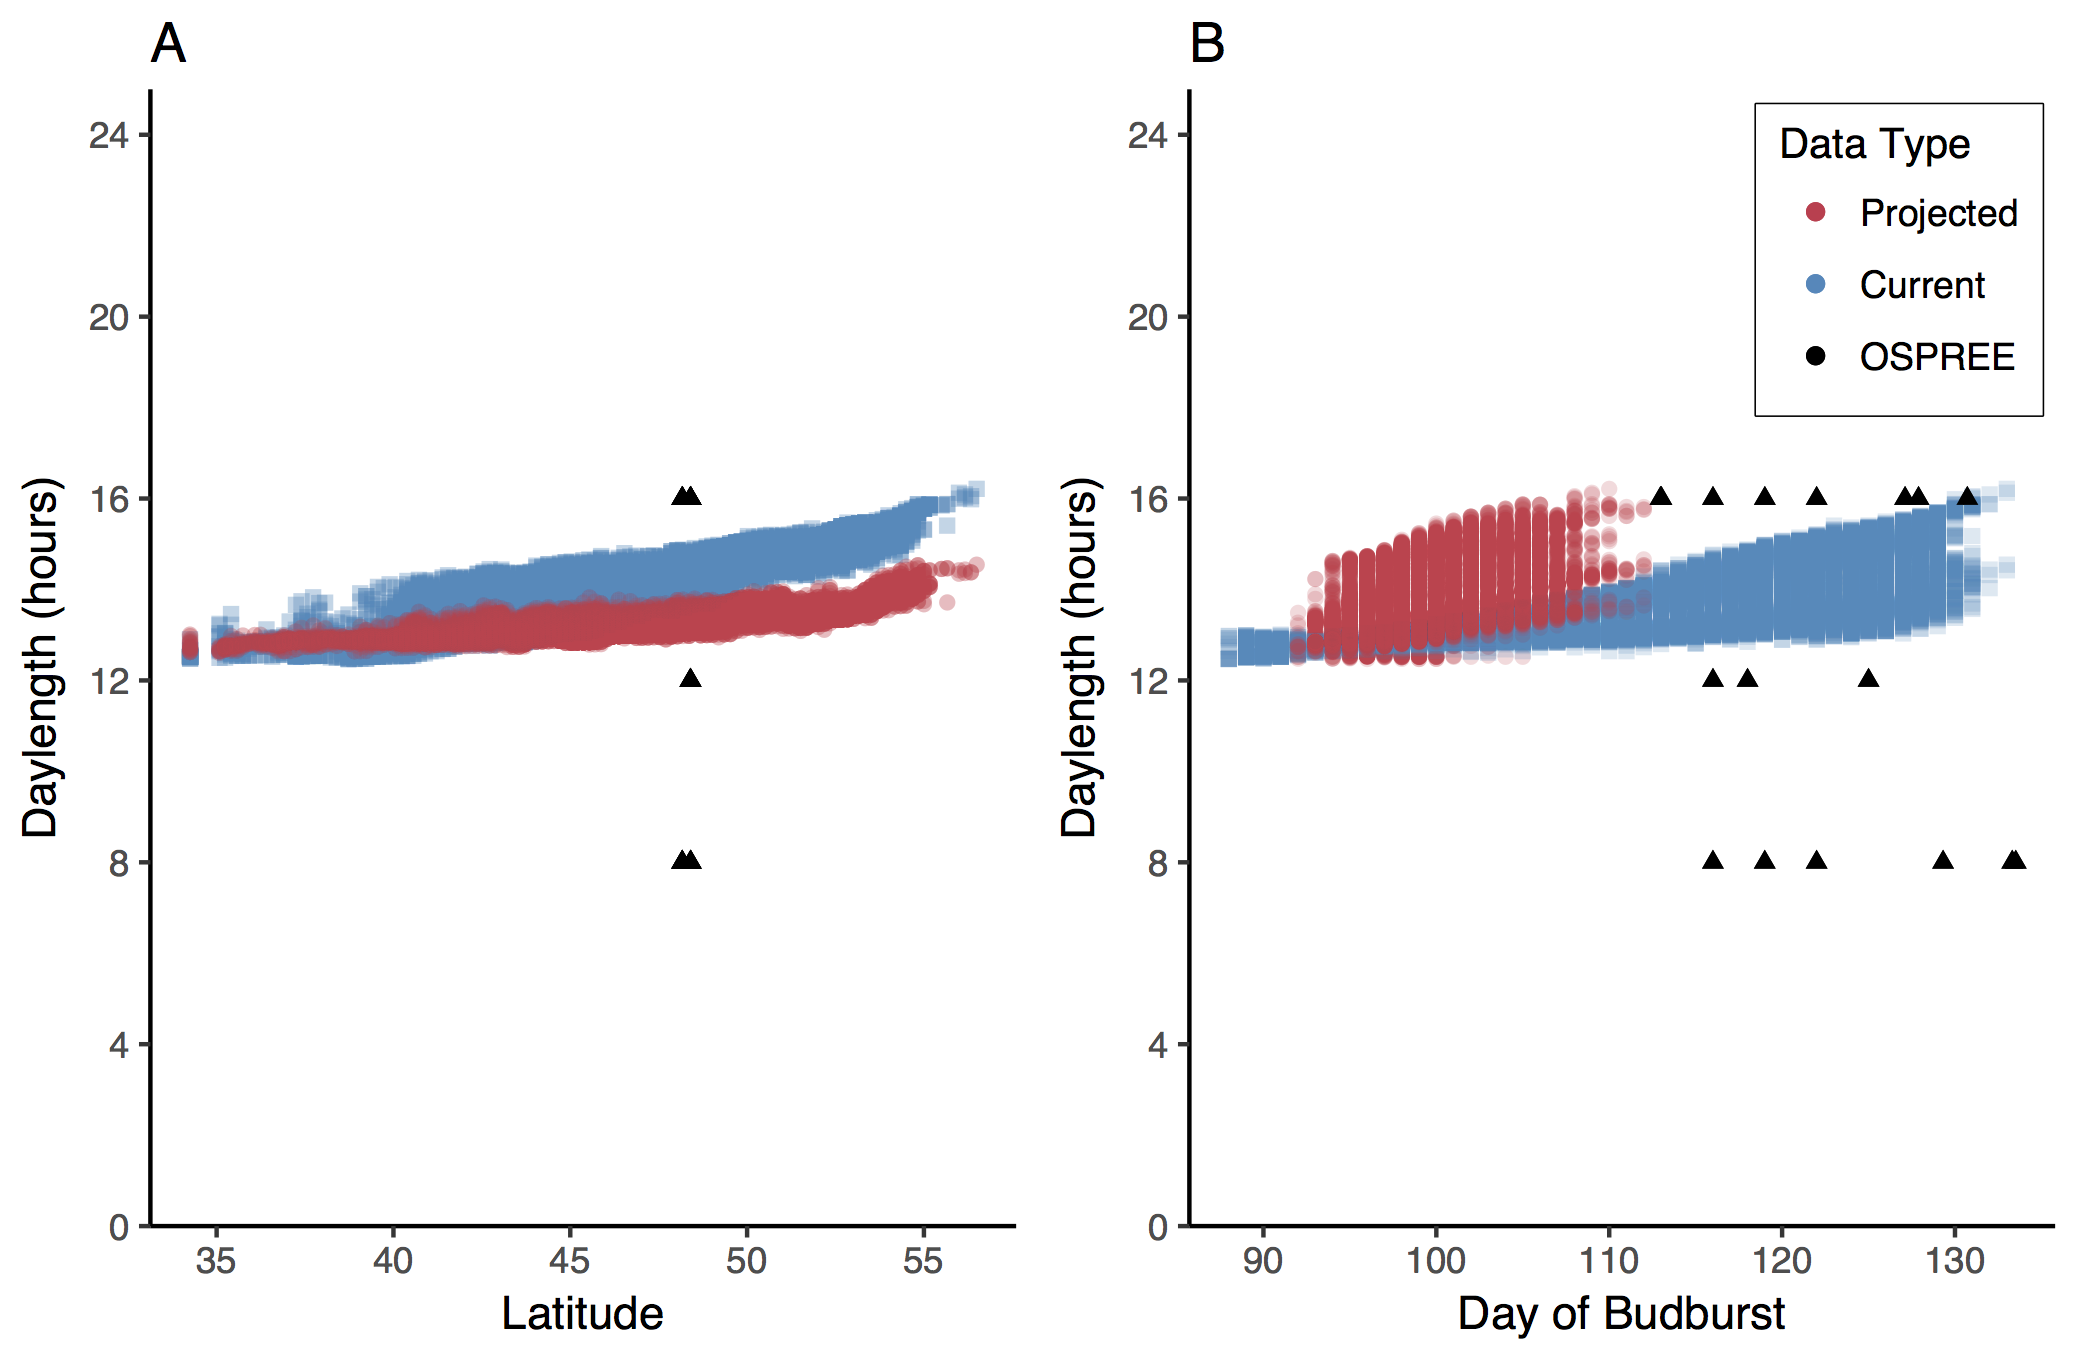
\includegraphics{/Users/aileneettinger/git/ospree/analyses/photoperiod/figures/2D_quercus_actual.pdf} 
\caption{\textbf{Experimental treatments of daylength in the OSPREE database, shown by latitude (A) and by day of budburst (B)} for \textit{Quercus robur}. For comparison, we show the daylength when budburst occurs in its current and projected ranges (A) and in its current range only, with expected shifts in phenology (B). Estimates and projections are from Phenofit \citep{duputie2015}.}
 \label{fig:quercus}
 \end{figure}
 
 \begin{figure}[p]
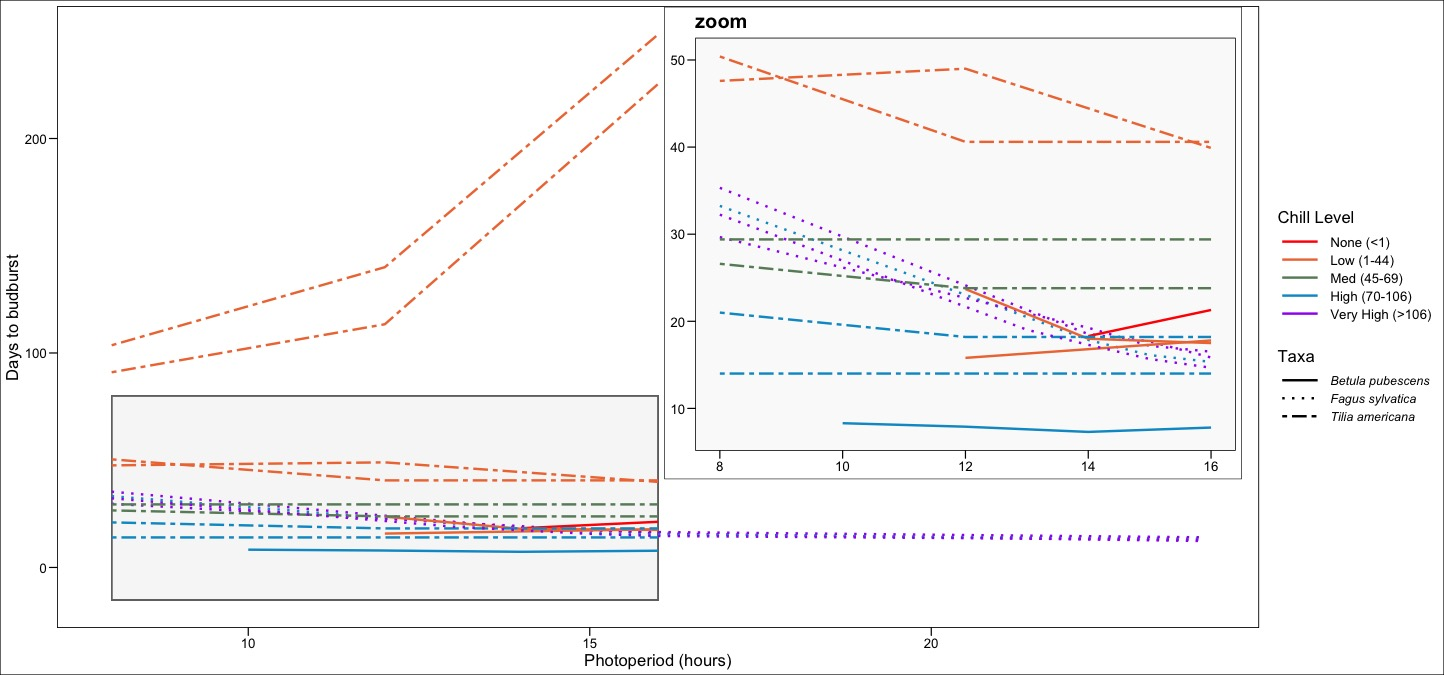
\includegraphics{/Users/aileneettinger/git/ospree/analyses/photoperiod/figures/Photo_curv_FINAL.jpeg} 
\caption{\textbf{Plant responses to changes in daylength vary across species and populations, and with the amount of chilling recieved}.}
 \label{fig:photocurve}
 \end{figure}
%%%%%%%%%%%%%%%%%%%%%%%%%%%%%%%%%%%%%%%%
\end{document}
%%%%%%%%%%%%%%%%%%%%%%%%%%%%%%%%%%%%%%%%
